A Python class that implements a PID controller for the satellite is shown below.
\lstinputlisting[language=Python, caption=satelliteController.py]{../control_book_public_solutions/_C_satellite/python/hw10/satelliteController.py}

Python code that implements the complete simulation is shown below
\lstinputlisting[language=Python, caption=satelliteSim.py]{../control_book_public_solutions/_C_satellite/python/hw10/satelliteSim.py}

Complete simulation code for Matlab, Python, and Simulink can be downloaded at \controlbookurl{http://controlbook.byu.edu}.


%A high-level Simulink diagram that implements the PID controller using output feedback is shown in Figure~\ref{fig:hw10_simulink_satellite}.
%\begin{figure}[hbt]
%  \centering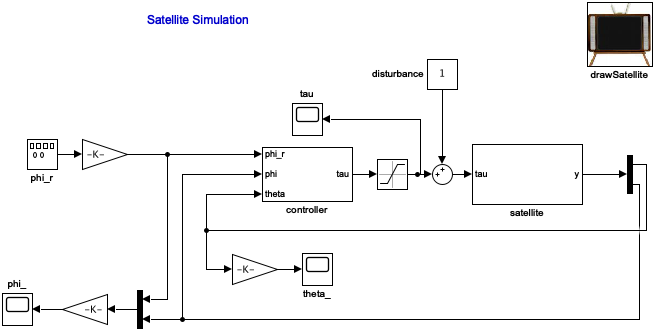
\includegraphics[width=0.8\textwidth]{6_design_studies/figures/hw10_simulink_satellite}
%  \caption{High level simulink diagram used for HW C.10}
%  \label{fig:hw10_simulink_satellite} 
%\end{figure}
%The Matlab/Simulink code for the controller is listed below.
%\lstinputlisting[language=Matlab, caption=satellite\_ctrl.m]{../control_book_public_solutions/_C_satellite/simulink/hw10/satellite_ctrl.m}


